%%%%%%%%%%%%%%%%%%%%%%%%%%%%%%%%%%%%%%%%%%%%%%%%%%%%%%%%%%%%%%%%%%%%%%%%%%%%%%%
%
% Tommy P. Keane
% Master of Science Thesis
% Department of Electrical and Microelectronic Engineering
% Rochester Institute of Technology
%
% April 2011
%
%
%
% Funded By: Lenel Systems Inc., A UTC Fire & Security Corporation
%
% Algorithm Intellectual Property Owned By: Lenel Systems Inc.
%
%
% http://www.tommypkeane.com
%
%%%%%%%%%%%%%%%%%%%%%%%%%%%%%%%%%%%%%%%%%%%%%%%%%%%%%%%%%%%%%%%%%%%%%%%%%%%%%%%

%%%%%%%%%%%%%%%%%%%%%%%%%%%%%%%%%%%%%%%%%%%%%%%%%%%%%%%%%%%%%%%%%%%%%%%%%%%%%%%
%
% CHAPTER 2
%
% SECTION 4: Mutual Information
%
%%%%%%%%%%%%%%%%%%%%%%%%%%%%%%%%%%%%%%%%%%%%%%%%%%%%%%%%%%%%%%%%%%%%%%%%%%%%%%%


%%%%%%%%%%%%%%%%%%%%%%%%%%%%%%%%%%%%%%%%%%%%%%%%%%%%%%%%%%%%%%%%%%%%%%%%%%%%%%%
% BEGIN DOCUMENT

Excellent texts to reference for this discussion, pertaining to its development or when in need of a deeper understanding of tnformation theory, are \cite{Reza1994}, \cite{MacKay2004}, \cite{Kullback1997}, and \cite{Cover2006}. The text by Cover and Thomas \cite{Cover2006} is an excellent reference for those with a prior understanding of information theory but are in need of a refresher, while the text by MacKay \cite{MacKay2004} is better suited for those unfamiliar with information theory or the application of probability theory. A lot of the following discussion is best referenced by \cite{Cover2006}.

\begin{figure}[h]
\centering
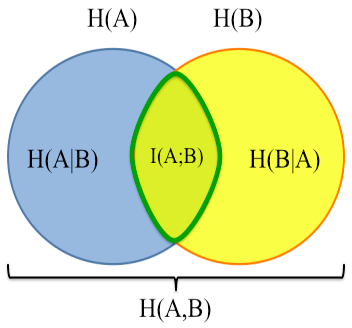
\includegraphics[height=.4\textwidth]{informationTheory}
\caption{Venn diagram of key measures in Information Theory}
\label{informationTheory}
\end{figure}

In a general case, mutual information can be understood as the measurement of the average shared determinism between two random variables; that is, how much does the probability of occurrence of one random variable portray about the probability of occurrence of another. In the case of digital images we are looking at discrete random variables, with their characterizing PMFs (probability of occurrence), and thus discrete entropy measures. Entropy, $H(A)$, is the measure of average randomness in a random variable and is used in the derivation of the mutual information formula. The following information theory terms to be described can be visualized in Figure \ref{informationTheory}. Calculating entropy for the random variable $A$ is shown in Eq. \ref{entropy}. Calculating mutual information in digital images makes it a discrete measure based on discrete random variables and their distributions. Whenever you have two random variables, you can generate a measure of their mutual information, conceptually, by measuring how their marginal entropies relate to their conditional entropy. Again, by referencing Figure \ref{informationTheory}, it is quite clear that there are several ways to determine the mutual information $I(A;B)$. To choose the most appropriate method for calculating mutual information, a view of mutual information applied to image registration can make this derivation much clearer, albeit this is conceptually going in reverse.

\begin{equation}
\label{entropy}
	H(A) = \sum_{i}{p_{A}(a_{i}) \log_{n}{\left(p_{A}(a_{i})\right)}}
\end{equation}

In beginning with two digital images, again with an example system image with 8-bpp and a single channel, the question of registration is: what pixels in image A are found in image B? A refinement of this question, thinking more in line with this research, is: what portions or regions, if any, from these images, have captured the same area of the scene? In general, as described in Section 1.2, the four stages of image registration typically deal with pixel correspondences. Once the correspondences are found, the corresponding pixel locations from one image are mapped to their equivalents in the other image, and that mapping is described as an invertible homography. The WFMI algorithm ultimately uses a discrete mutual information measure to determine the correspondences required to register the two images, but it does not look directly for pixel-to-pixel correspondence.

An 8-bpp $\mathfrak{m} \times \mathfrak{n}$ image is a bounded  set of $\mathfrak{m} \cdot \mathfrak{n}$ intensity values distributed randomly in the interval of [0,255]. Corresponding this set to another image, \ie{ }another data set, requires some mathematical measure that is based on mathematical attributes of the data sets themselves, \ie{ }their PMFs. Given two digital images, their two intensity histograms can be found, then normalized to generate their image PMFs (also called the marginal PMFs), and then their marginal entropies can be determined through Eq. \ref{entropy}.

The measure of entropy is presenting the minimum number of bits required to encode or losslessly transmit the $\mathfrak{m} \cdot \mathfrak{n} \cdot \mathfrak{p}$ random pixels of an image. If they are completely random, the entropy is comparably large, but if the data is completely deterministic the entropy approaches 0. The mathematical determination of this randomness measure is essentially characterizing the amount (or lack thereof) of redundancy in the data. This gives a metric of encoding efficiency but not a means of encoding. Therefore it is best to understand entropy as a bounding metric, since it presents the minimum amount of bits for encoding in an ideal situation, which is often not achievable, or in the case of non-integer results, it is not physically possible (as we cannot realistically transmit $3.2$ bits, but that is a potentially valid entropy). By equations \ref{entropy} and \ref{PMF}, one can take the distribution of a data set and determine its entropy. Classically, $n$ is taken to be 2, so as to create a value $H(A)$ measured as the total number of unique bits required to losslessly encode the data. Equation \ref{PMF} is the equation for generating the image PDF.

\begin{equation}
\label{PMF}
	p_{A}(\bf{a})=h_{A}(\bf{a}) \cdot \left(\sum_{i}{h_{A}(a_{i})} \right)^{-1} = \frac{h_{A}(\bf{a})}{\mathfrak{m}\cdot\mathfrak{n}}
\end{equation}


Now stepping back to the digital image as a data set, it is clear that a measure of entropy can be determined for each image. Then joint and conditional probability densities between the images can be determined from joint and marginal histograms. For the bivariate histogram, the $(n_{i},p_{j})${-}bin's value means: there are this many pixels where image A has intensity relating to index $n_{i}$ and image B has intensity relating to index $p_{j}$ at the same spatial location (given images of the same size). In the case of generating the bivariate histogram between an image and itself, the result is an $\mathfrak{m} \times \mathfrak{n}$ ``identity'' matrix since an image will only have a value relating to index $n_{i}$ where itself also has the value relating to index $p_{j}$ when $i \equiv j$. For example, given $h_{AB}(0,2)=4$, then what is known is that somewhere in image A there are at least 4 pixels with intensity values in the range of bin 0, and there are at least 4 pixels in image B with intensity values in the range of bin 2, and that only 4 of those pixels in each image are in the exact same spatial locations within the images. That is all that is known and can be extracted from only the bivariate histogram. It too encodes spatial data that cannot be uniquely decoded.

This is a major factor in understanding the application of mutual information, because as is shown in Equation \ref{MutualInformation}, the mutual information is developed from the joint and marginal histograms.

\begin{equation}
\label{MutualInformation}
	I(A,B) = \sum_{j}{\sum_{i}{p_{AB}(a_{i},b_{j}) \log_{2}{\left( \frac{p_{AB}(a_{i},b_{j})}{p_{A}(a_{i})p_{B}(b_{j})}\right)}}}
\end{equation}

\noindent What is immediately apparent is that if the product of the marginal distributions is equal to the joint distribution, then the mutual information is zero. When a joint distribution is equivalent to the product of the marginal distributions the two random variables are said to be independent. So when the random variables are independent, then they will have no mutual information. And again, mutual information is, at its heart, a measure of randomness, i.e. an entropy measure. Joint entropy depicts how random two images are, jointly, by denoting the number of bits required to encode them. Mutual information denotes how much the random information in A can convey knowledge about the random information in B. Thus in the further development of this algorithm the normalized mutual information value presented in Equation \ref{NormalizedMutualInformation} will be used, as developed by the work in \cite{Yao1999} which characterized it as a symmetric and normalized measure.

\begin{equation}
\label{NormalizedMutualInformation}
	I(A,B) = \left( \frac{2}{H(A) + H(B)}\right) \cdot \sum_{j}{\sum_{i}{p_{AB}(a_{i},b_{j}) \log_{2}{\left( \frac{p_{AB}(a_{i},b_{j})}{p_{A}(a_{i})p_{B}(b_{j})}\right)}}}
\end{equation}

\noindent What this provides is a mutual information measure that is dependent only upon the two images, A and B, and their total number of applicable pixels.

Now there is a single value result for any comparison of distributions, with high values meaning similar distributions and values approaching zero (as it is a non-negative measure) meaning dissimilar distributions. Since images or regions of images can be seen as random variables characterized by their distributions, then they too can be compared in this manner. Ultimately the question here will be how to generate the distributions, meaning, what data is used from the images to develop the histograms, and why it is done for these surveillance situations? Note that this is a distribution measure, not an element-by-element measure.


%%%%%%%%%%%%%%%%%%%%%%%%%%%%%%%%%%%%%%%%%%%%%%%%%%%%%%%%%%%%%%%%%%%%%%%%%%%%%%%
% END OF DOCUMENT

